\documentclass[11pt] {article}
\usepackage{amssymb}
\usepackage{amsmath}
\usepackage[colorlinks=true]{hyperref}
\usepackage[scaled=2.5]{helvet}
\setlength{\parsep}{20pt}
\usepackage{geometry}
\geometry{letterpaper}            
\usepackage{graphicx}					
\usepackage{amssymb}
\usepackage{caption}
\usepackage{subcaption}

\newcommand{\bs}[1] {\boldsymbol{#1}}

\begin{document}
\title{Asymmetric three point bending test with three holes}
%\author{Kaushik Vijaykumar}
%\date{January 12, 2015}
\maketitle
Experimental crack path of three point bending experiment of an asymmetrically notched-beam with three holes is given in \cite{bittencourt1996quasi}. The geometry and the loading conditions can be seen in Figure~\ref{Fig1}. The Youngs modulus $E$, is 20.8 $GPa$, Poisson's ratio $\nu$, is 0.3 and the fracture toughness $g_c$, is 1 $N/mm$. The geometry is constrained on the bottom edge by fixed boundary condition, 1 unit from the left edge and a roller boundary condition 1 unit from the right edge. The geometry is subjected to a load point displacement $u$ at the center of the top edge i.e., at a distance of 10 units from the left edge. 
\begin{figure}[ht!]
	\centering
	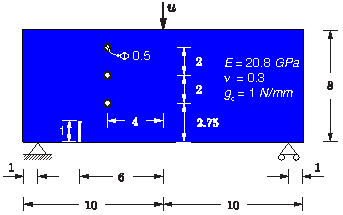
\includegraphics[width=0.75\textwidth]{3_hole_bend.pdf}
	\caption{The geometry and the loading conditions is shown in (figure adapted from \cite{miehe2010phase}). The diameter of the holes in indicated by $\phi$, and is equal to 0.5 units.}
	\label{Fig1}
\end{figure}

\bibliographystyle{plain}
\bibliography{Ref}
%\begin{thebibliography}
%\end{thebibliography}
%
\end{document}
